% Import the subfiles package, which allows the document to be
% split into smaller subfiles for easier management
\documentclass[../main.tex]{subfiles}

\begin{document}
\pagebreak
\section{Background}

This chapter presents the definition of the problem,
scope of the problem,
different solutions related to the problem and
why this solution is chosen.

\subsection{The \gls{medicolbox}}

the \gls{medicolbox} is the medicine colletion part of Medretur’s solution for collecting medicine in an effort to prevent medicinal waste and damage.

the \gls{medicolbox} is a box made by $8$ mm thick aluminium plates. It is $600$ by $600$ mm wide and $600$ mm high.
On the side of it is a removable cart held together with internal locking mechanisms in steel designed to not pose a weak point on the box.

On top of this box is bolted tight a wedge shaped lid, also $600$ by $600$ mm wide.
The wedge shaped lid is $600$ mm high on the tallest section and $200$ mm high on the lowest section.
on top of the lid is a touch screen posing as the \gls{hmi} and an opening designed to allow you to insert some medications for internal mechanisms to sort.

\begin{figure}[htbp]
    \centering
    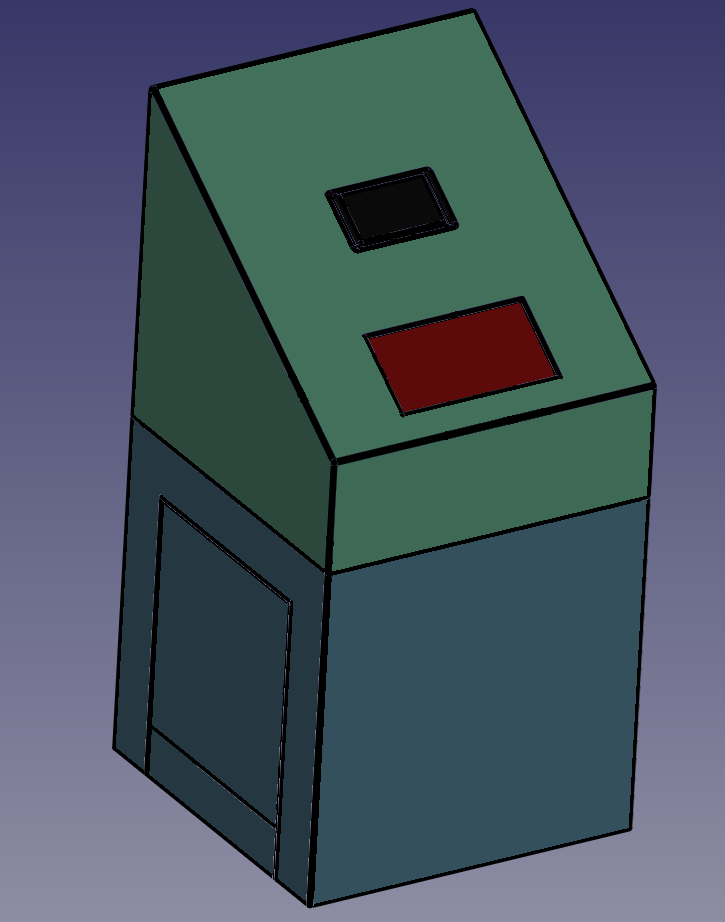
\includegraphics[width=0.5\textwidth]{resources/images/MediColBox.png}
    \caption{render of the \gls{medicolbox} from before it was built}
    \label{fig:medicolbox_render}
\end{figure}

The total weight of the \gls{medicolbox} is $86$ kg and the aluminium casing has been tested to sustain repeated impacts with an estimated force of $8 000$ 
(this has been meassured using an internal accelerometer,
meassuring the maximum total acceleration registered during the impact and multiplying that acceleration with the mass of $86$ kg.)
In general Aluminium is a somewhat soft metal, so impacts may deform the box, but will most likely not manage to yield access to the inside of the box.

Aluminium, being a soft and malleable material, is somewhat easy to cut, making it weak to the "universal key" constituting of a battery powered angle grinder with specialised cutting discs.


\subsection{Definition of the problem}
The problem is \gls{intrusion}, but is what is \gls{intrusion}?
According to Merriam-Webster,
an online English dictionary,
\gls{intrusion} is a noun and is defined in this context as:

\enquote{the act of intruding or the state of being intruded}\cite{definition-intrusion}

especially:

\enquote{the act of wrongfully entering upon, seizing,
or taking possession of the property of another}\cite{definition-intrusion}

In the context of the \gls{medicolbox}, the word
"\gls{intrusion}" refers to attempts on breaking collection system
in an effort to gain access to the disposed medicines stored inside.
The \gls{medicolbox} contains medications that are
expired or no longer needed, which can pose a danger to
individuals if they are not disposed of properly\cite{peds}. 

The improper disposal of medications can lead to
environmental contamination, harm to human health,
and the potential for misuse.

The black market for medications also presents a criminal incentive
to break into the collection system and steal the medications for resale.
Additionally, there are individuals who may be addicted to certain
medications and would seek to gain access to them for personal use.

Therefore, it is crucial to ensure that the \gls{medicolbox} is secured
and protected from \gls{intrusion} attempts to prevent the
tampering or theft of medications.

This requires the implementation of effective detection
and deterrent measures to identify and stop
\gls{intrusion} attempts in real-time.

To intrude into the \gls{medicolbox} in an attempt to get access to
the medicines inside, it will be necessary to get through
the outer metal shell. The metal shell, in this context,
is a type of mechanical barrier,
separating the outside from the inside.

Most types of \gls{intrusion} attempts can be simplified to the contents of
(Table \ref{tab:TypesOfIntrusionAttempts}).

\begin{table}[htbp]
    \centering
    \caption{Types of Intrusion Attempts}
    \label{tab:TypesOfIntrusionAttempts}
    \begin{tabular}{|l|p{10cm}|} \hline
        \textbf{Intrusion Attempt} & \textbf{Description} \\ \hline
        Cutting through the shell & This type of intrusion attempt involves using tools such as saws or angle grinders to physically cut through the outer metal shell of the \gls{medicolbox}. It is a relatively straightforward method that can be quickly executed if the intruder has the necessary tools and equipment. \\ \hline
        Forcing apart the shell & Forcing apart the shell refers to attempts to pry open or force the outer metal shell of the \gls{medicolbox} using tools such as pry bars or similar implements. This method relies on applying excessive force to separate the components of the shell and gain unauthorized access. \\ \hline
        Exploiting the shell & Intruders may attempt to unlock the shell using various exploits, such as lock picking tools, brute force attacks, or electronic hacking techniques. These methods involve manipulating the lock or electronic components of the shell's locking mechanism to gain access without proper authorization. \\ \hline
    \end{tabular}
\end{table}

Cutting through or forcing apart the outer metal shell of
the \gls{medicolbox} are relevant \gls{intrusion} attempts because
they can potentially compromise the security of the contents inside,
which are the expired or unused medications.
Unauthorized access to these medications can pose a
serious risk to public health and safety, as they may be misused,
abused, or sold illegally.

Cutting through the shell can be done using power tools such as
saws or angle grinders, while forcing apart the shell
can be done using a pry bar or a similar tool.
These methods of \gls{intrusion} are relatively easy to carry out
and can be completed quickly,
especially if the intruder has the necessary tools and equipment.

To prevent cutting or forcing open the shell,
physical barriers can be implemented.
These can include tamper-proof screws or bolts,
reinforced steel plates, or alarm systems.
Tamper-proof screws or bolts can be used to secure the outer shell,
making it difficult for intruders to unscrew or remove them.
Reinforced steel plates can be placed over the shell to
increase its strength and make it more difficult to cut or force apart.
Alarm systems can be used to alert authorities and deter
intruders from attempting to break into the \gls{medicolbox}.

In addition to physical barriers,
other security measures can be employed to prevent \gls{intrusion} attempts.
These can include access control systems such as key card readers
or biometric scanners,
security cameras to monitor the area around the \gls{medicolbox},
and regular security patrols or checks.

It is important to note that no security measure is completely foolproof,
and determined intruders may still be able to find
ways to breach the security of the \gls{medicolbox}.
However, by implementing a combination of
physical and electronic security measures,
the risk of \gls{intrusion} can be significantly reduced,
and the contents of the \gls{medicolbox} can be better protected.

Exploit-based \gls{intrusion} attempts on the \gls{medicolbox} could involve
attempts to bypass or manipulate the locking mechanisms
in order to gain unauthorized access to the contents inside.
These \gls{exploit} could include using lock picking tools,
\enquote{brute force attacks}, or electronic hacking techniques.

Lock picking tools are designed to manipulate the internal workings
of locks in order to unlock them without using the key.
Brute force attacks involve attempting to force the lock
by applying excessive force, such as hitting
or kicking the lock or using a tool to pry it open.
Electronic hacking techniques may involve attempting to manipulate
the electronic components of the lock,
such as by intercepting signals sent between the
lock and its control system
or by exploiting vulnerabilities in the lock's firmware or software.

Exploit-based \gls{intrusion} attempts are difficult to detect and prevent
because they may not leave physical evidence and may not
trigger alarms or other security measures.
In addition, these types of attacks may be carried out by individuals
with specialized knowledge or equipment,
making them more difficult to defend against.

The potential consequences of an exploit-based \gls{intrusion}
attempt on the \gls{medicolbox} could include unauthorized access to
the expired or unused medications inside,
which could lead to harm to individuals who consume or misuse them.
In addition, successful exploitation of
the \gls{medicolbox}'s security measures could compromise the
overall security of the system,
potentially leading to further unauthorized access
or theft of medications.

To prevent exploit-based \gls{intrusion} attempts,
it is important to implement strong physical
and electronic security measures,
as well as regular monitoring and maintenance of the security systems.
This can include using tamper-proof locks and security cameras,
implementing access control systems with strong authentication mechanisms,
and regularly updating the firmware and software of
the locking mechanisms to address any known vulnerabilities.
It is also important to regularly review and update
security policies and procedures to ensure that
they are up-to-date and effective in addressing new threats and risks.

the last point in the list implies there is something
unpredicted and unplanned, so this project will
recommend this for future studies
instead of covering it in this study.

the project will therefore focus on detecting
and deterring cutting and forcing open the shell.

There are several detection and deterrence methods
that can be used to prevent cutting and forcing open the shell of
the \gls{medicolbox} as specified (Table \ref{tab:PotentialSecurityMeasuresForMediColbox}).

\begin{table}[htbp]
    \centering
    \caption{Potential Security Measures for MediColbox}
    \label{tab:PotentialSecurityMeasuresForMediColbox}
    \begin{tabular}{|l|p{10cm}|} \hline
        \textbf{Security Measure} & \textbf{Description} \\ \hline
        
        Physical Barriers &
        As mentioned earlier,
        physical barriers such as tamper-proof screws,
        reinforced steel plates,
        or alarm systems can be used to prevent unauthorized access to
        
        the \gls{medicolbox}.
        These barriers can deter intruders from attempting to
        break into the box and can also alert authorities to
        any intrusion attempts. \\ \hline
        
        Inertial Measurements &
        Utilizing an \gls{imu} in the
        sensor card to detect any changes in the box's orientation or
        movement, providing additional data for
        intrusion detection and prevention. \\ \hline
        
        Motion Sensors &
        Motion sensors can be placed around the
        \gls{medicolbox} to detect any movement or
        activity in the surrounding area.
        If an intruder attempts to cut or force open the shell,
        the motion sensors will detect their movement and
        trigger an alarm,
        alerting authorities to the intrusion attempt. \\ \hline
        
        Video Surveillance &
        Video cameras can be installed around the \gls{medicolbox} to monitor any activity in the surrounding area. The footage can be monitored in real-time by security personnel, who can alert authorities to any intrusion attempts. \\ \hline

        Smart Locks &
        Smart locks can be used to secure the \gls{medicolbox}, using electronic authentication mechanisms such as biometric scanners, keycard readers, or passwords. These locks can be integrated with other security measures, such as motion sensors or video surveillance, to provide additional layers of security. \\ \hline
        
        GPS Tracking &
        GPS tracking technology can be used to monitor the location of the \gls{medicolbox} and track any unauthorized movement or tampering. This can help to deter theft or unauthorized access to the box. \\ \hline
    \end{tabular}
\end{table}


Existing technologies that can be adapted for use in the \gls{medicolbox}
include tamper-proof screws or bolts, reinforced steel plates,
alarm systems, motion sensors, video cameras, smart locks,
and GPS tracking devices.
These technologies can be integrated into the overall system
by connecting them to a central control system or security platform,
which can monitor and manage the various security measures in real-time.

Overall, by implementing a combination of
physical and electronic security measures,
the risk of cutting and forcing open the shell of the \gls{medicolbox}
can be significantly reduced,
and the contents of the box can be better protected.

\end{document}
